\chapter{宇宙インターネットにおけるDTN技術とそのルーティング}
\label{chap:prerequisite_knowledge}

\section{近年の宇宙開発の進展}
宇宙開発は近年大きく進展している。1970年代に米ソによって月探査が進展した後、その後月面、特に有人による探査は中断されていたが、
2004年にブッシュ大統領は米国の新宇宙政策を発表し、2020年までに米国が再び宇宙飛行士を月面に送り、有人滞在施設の建設することを提唱した。\cite{久保田2009}
この計画は実際には中断されたものの、2017年にトランプ大統領が有人月探査・火星探査を進める大統領令に署名し、2019年にアルテミス計画として発表された。\cite{nasa2020}
2020年には「アルテミス計画を含む広範な宇宙空間の民生探査・利用の諸原則について、関係各国の共通認識を示すこと」を目的にアルテミス合意\cite{artemis_agreement1}も成立し、
当初日本・アメリカ・カナダ・イギリス・イタリア・オーストラリア・ルクセンブルク・アラブ首長国連邦の8カ国が参加した。\cite{artemis_agreement2}
加盟国はその後増加し、2024年時点で40カ国である。\cite{artemis_agreement3}
このように近年宇宙開発は急激に進展しており、その進展について以下の\ref{月・火星の探査計画}、
、\ref{深宇宙の探査計画}、\ref{民間事業者の宇宙事業への参画}の三つの視点から述べる。


\subsection{月・火星の探査計画}
\label{月・火星の探査計画}
このセクションでは、西側のアルテミス計画、及び中露の月・火星探査計画とそのタイムラインについて詳述する。

\subsection{深宇宙の探査計画}
\label{深宇宙の探査計画}
このセクションでは、火星以遠の探査計画、特に小惑星探査やそのほか木星土星の衛星探査についても詳述する。

\subsection{民間事業者の宇宙事業への参画}
\label{民間事業者の宇宙事業への参画}
このセクションでは、2000年代の民間事業者の宇宙事業への参入について詳述する。
特に、スペースX、ブルーオリジン、ヴァージンギャラクティックなどの宇宙への輸送能力をもつ企業の成長について述べる。
宇宙ビジネスの事業規模の拡大を示すとともに、今後地球軌道でのビジネスだけでなく、月・火星でのビジネスも進展し、
そこでの通信需要が生まれるという話を記述する。
メモ:JAXAのイノベーションハブについても述べる

\section{宇宙通信におけるインターネット技術の適用可能性}
\label{section:宇宙通信におけるインターネット技術の適用性}
これらの宇宙開発計画に伴い、 月・火星の地表及びその近傍の空間に多くの人や宇宙機、その他機材が存在するようになり、
天体内・天体間での通信需要が大きくなることが予想される。 
従来までの宇宙ミッションにおいて宇宙のノードと地球との通信は、 地球上にある各国の大型アンテナを利用し、 一対一の通信を行っていた。
しかしこのような計画でノードの数が増加する場合、通信ニーズに対応するためには宇宙にも多対多のノードで通信が可能な宇宙インターネットが必要となる。 
これに向け、既存のインターネットの技術を宇宙インターネットに向け改良し活用することが検討されているが、
当然ながら宇宙環境は地球とは環境が大きく異なり、特に以下の部分に関して考慮が必要となる。

\section{通信における宇宙の環境}
\label{section:通信における宇宙の環境}
宇宙における通信やネットワークに関して、地球とは次のような大きな違いが存在する。


\subsection{大きな遅延のある通信環境}
\label{subsection:大きな遅延のある通信環境}
宇宙での通信は既存のインターネットにおける通信の遅延に比較して非常に大きい。
東京-ニューヨーク間であれば、伝搬遅延のみを考慮した場合、片道50ms以内で通信が可能である一方、宇宙における通信の際には地球月間でも片道1。3秒、
地球火星間では太陽に対する2天体の公転の状況によって変動するが最大20分程度の遅延が想定されている。
End-to-EndでTCPを用いた通信を行う際には、 3-way-handshakeなどを含めこれらの天体間を複数回往復する通信を行う必要があり、 
遅延はさらに大きな時間になる。 
\cite{McBrayer2022}


\subsection{ネットワークトポロジーの変動と間欠的接続}
\label{subsection:ネットワークトポロジーの変動と間欠的接続}
宇宙のインターネットにおいて、ネットワークを構成するノードには多くの宇宙機が含まれている。
これらのノードは当然ながら宇宙空間での位置が常に変化しており、
 天体の影に入るなどで断絶が頻繁に起こる。 

\section{Delay and Disruption Tolerant Networking(DTN)}
これらの宇宙環境におけるインターネットのコンセプトとして、Delay and Disruption Tolerant Networking(DTN)が
が構想されている。DTNの中心となる技術の一つにRFC9171\cite{rfc9171}で標準化されたBundle Protocol(BP)があり、 
BPでは通信されるデータはバンドルという可変長のデータとして転送される。 
中間ノードでは経路上の次のノードへ転送可能なタイミングまでバンドルを蓄積することが可能になっているため、 
End-to-Endの通信疎通性が確保できていない場合でも、 この蓄積による転送を行うことにより断絶に強い通信ができる。
またトランスポートレイヤにUDPなどのプロトコルを用いることで、 比較的遅延を抑えて通信することもできる。\cite{bundle_protocol_architecture}

\begin{figure}[tbh]
    \centering
    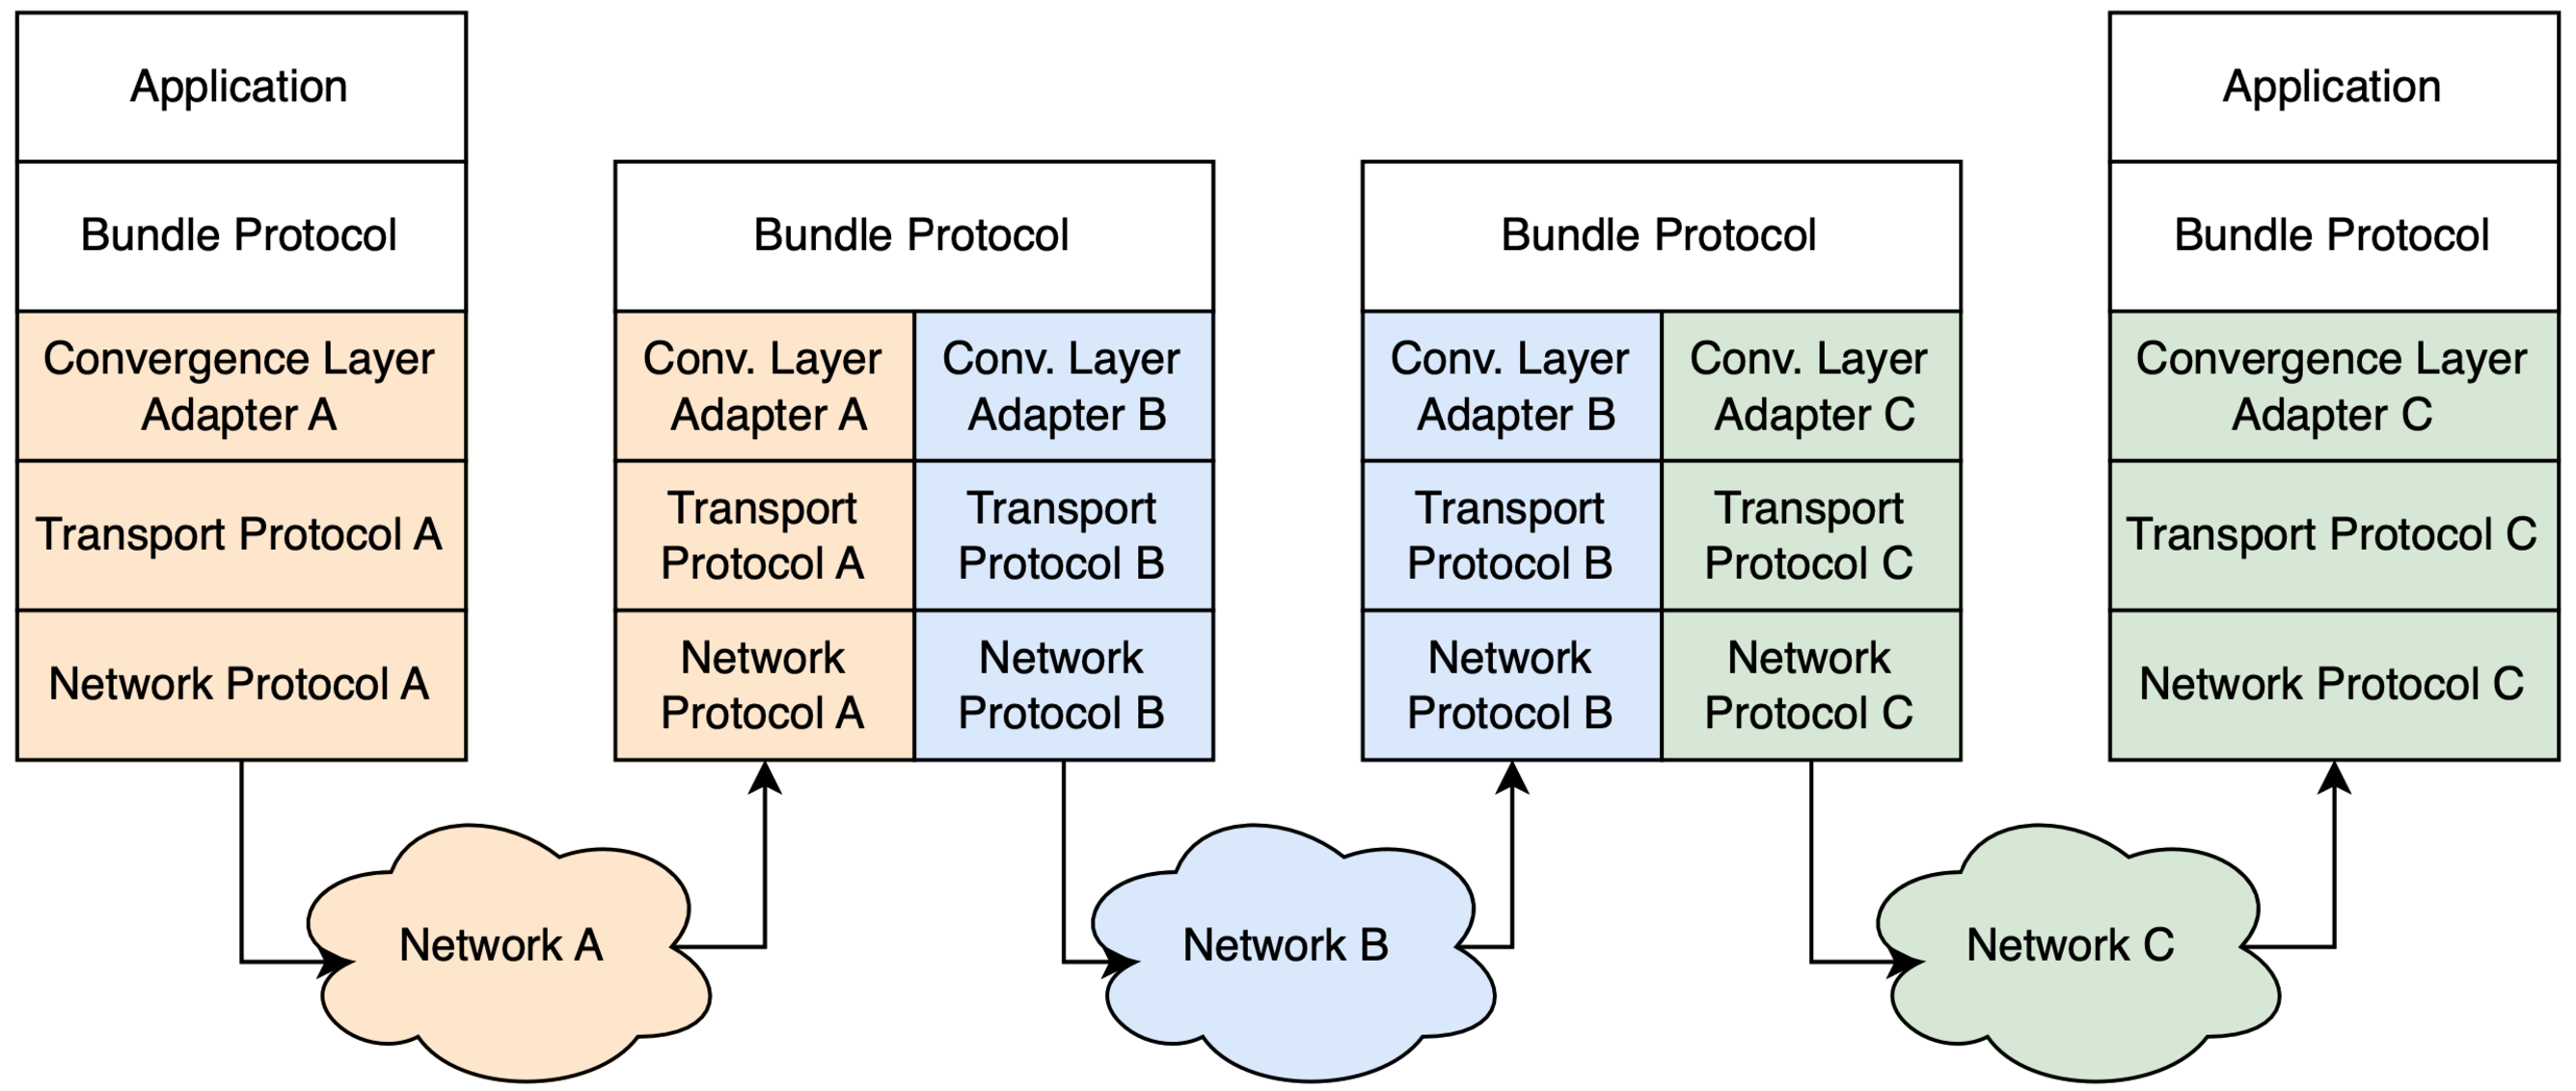
\includegraphics[width=0.7\textheight]{img/dtnprotocolstack.pdf}
    \caption{DTNを搭載したノード間のみでの通信}
    \label{fig:dtnprotocolstack}
    \begin{minipage}{\textwidth}
        \raggedright
        参考文献\cite{bundle_protocol_architecture}Figure1より引用。図中のConvergence Layer(CL)については\ref{subsection:Convergence LayerとLTP}で説明する.
    \end{minipage}
\end{figure}

\subsection{宇宙におけるDTN}
DTNは当初惑星間インターネットのアーキテクチャのコンセプトとして構想された。しかしRFC 4838\cite{rfc4838}において、
Delay Tolerant Networkingという言葉を使用した頃から、地上無線ネットワークへの適用も構想されるようになった。
これらの環境と宇宙環境でのDTNの大きな違いとして、通信機会のタイミングが挙げられる。
\ref{subsection:Contact Graph Routing}でも述べるが、
宇宙環境でのDTNにおいてはノード間の通信機会は全て予測可能なものである一方、
地上無線ネットワークでの通信機会は予測が難しいものであり、そのためルーティングの手法なども異なる。
本研究では宇宙のインターネットにおけるルーティング手法に注目しているため、以後は地上無線ネットワークにおけるDTNではなく、
宇宙インターネットで用いるDTNについて議論する。

\subsection{Bundle Protocol}
\label{subsection:Bundle Protocol}
上記でも述べたBPは、DTNにおける主要な通信技術で遅延・断絶が起きやすい環境でデータを確実に伝送するために設計された。
このバンドルは、 送信元から目的地までの途中で複数の中継を経ても、全体としてデータを確実に届けるためのものである。 
また、このプロトコルは「ストア&フォワード」方式を利用しており、 各中継ノードが受け取ったバンドルを一時的に保存し、 
次のノードと通信できるタイミングが来るまで待機する。 これにより、通信が一時的に途絶えてもデータが失われることなく、 次のノードへと送信される。

\subsection{IPN address}
\label{subsection:IPN address}
IPNアドレス(Interplanetary Networking Address)は、 DTN環境で使用されるアドレス形式で、
宇宙通信のためのネットワーク識別とエンドポイントの識別を可能にするものである。 従来のインターネットプロトコルアドレス(IPアドレス)は、
リアルタイムでの通信や短い遅延を前提とした設計であるため、 宇宙空間における遅延や断絶が発生する環境では適切に機能しない。
DTNのアーキテクチャは、 これらの遅延や断絶を前提としており、 IPネットワークとは異なる方法でデータを伝送するため、
IPNアドレスが必要とされている。 さらに、 IPNアドレスは地上のインターネットや宇宙のネットワークなど、
異なるアドレッシングスキームを持つネットワークの統合する役割としても機能する。

IPNアドレスは「ipn:ノード番号. サービス番号」という形式で記述され、 これにより特定の宇宙船や装置が個別に識別される。 

\subsection{Convergence LayerとLTP}
\label{subsection:Convergence LayerとLTP}
DTNでは多様なプロトコルがトランスポートレイヤ以下の層で使用することを想定しており、 図\ref{fig:dtnprotocolstack}中のConvergence Layerは
それらの違いを吸収することを目的としている。 Convergence Layer Protocol(CLP)としては、 
利用する下位レイヤプロトコルにより、
\begin{itemize}
    \item TCP-based CLP (TCPCL)
    \item User Datagram Protocol (UDP)-based CLP (UDPCL)
    \item Saratoga CLP
    \item Licklider Transmission Protocol (LTP)-based CLP (LTPCL)
\end{itemize}
などがある。
LTP\cite{rfc5326}はコンバージェンスレイヤのプロトコルの一つであり、 再送制御の機能も実装している。
LTPをコンバージェンスレイヤに用いる場合、 トランスポートレイヤにUDPを用いることがあるほか、 
宇宙での通信においてLTPが直接リンク層にアクセスすることも想定されている。
\subsection{既存のDTN実装}
既にいくつかの研究機関などによりDTN技術を実装したソフトウェアがリリースされている。 いくつかの例を以下に示す。 
\begin{itemize}
    \item Interplanetary Overlay Network DTN(ION-DTN): NASA/JPL
    \item HDTN : NASA/Glenn research center
    \item DTN ME : Marshall Space Flight center
    \item \textmu D3TN : D3TN GmbH
    \item IONe : Experimental ION Scott Burleigh United States 
    \item DTN7/Go : University of Marburg German
\end{itemize}
これらのDTNソフトウェアは、 基本的に通信内容からバンドルへのエンコード・デコード、 
中間ノードでのバンドルのままでの蓄積転送を可能にしているが、 
Convergence Layerが対応しているトランスポートレイヤプロトコルの種類などの点で異なる。 
これらの実装についての比較についてを表\ref{fig:chart_dtn_implementations}に示す。   
\begin{table}[tbh]
    \centering
    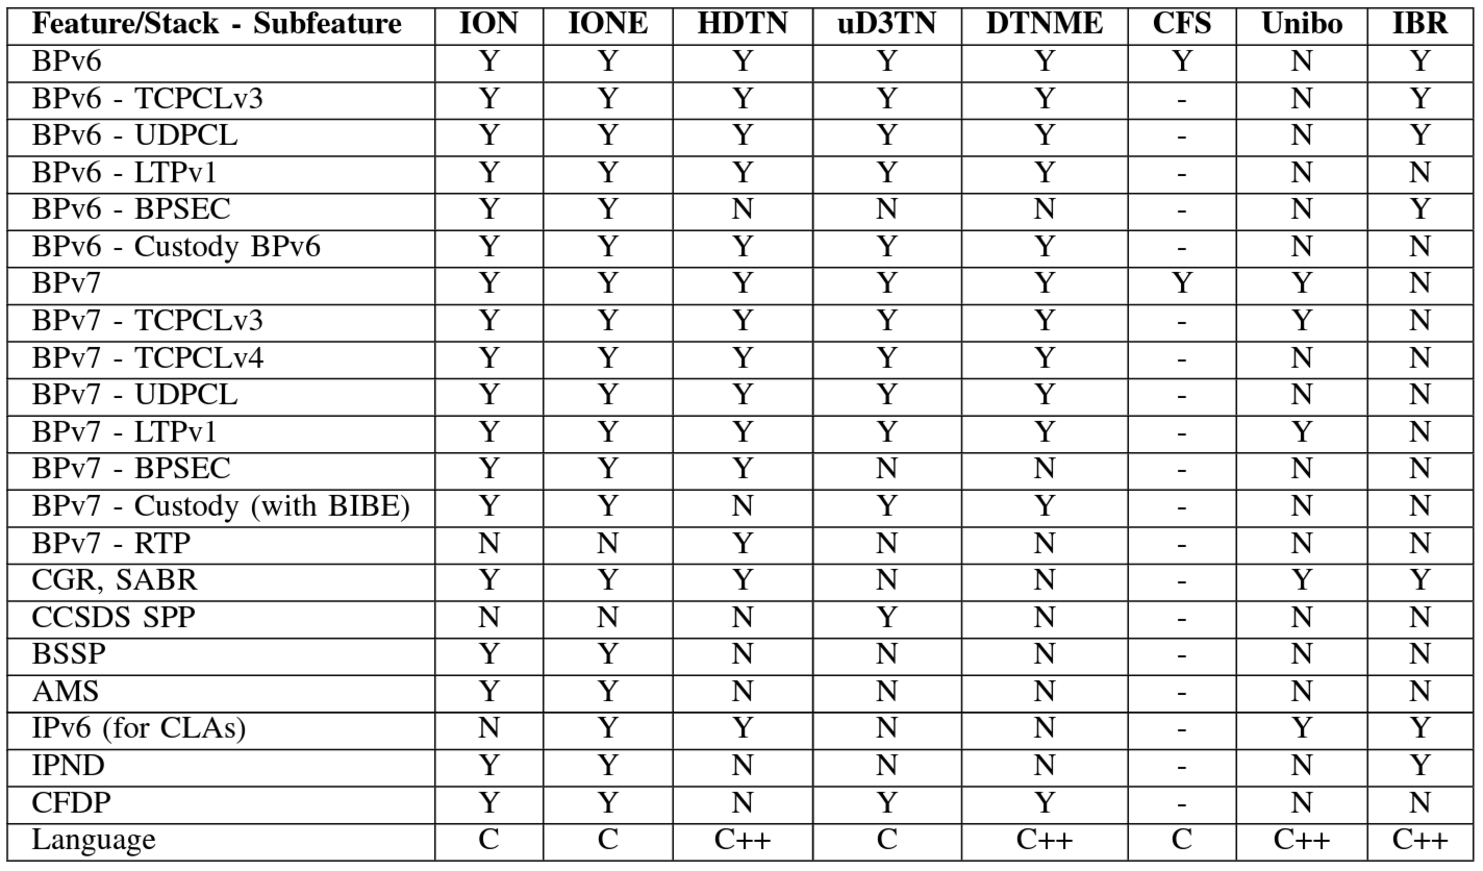
\includegraphics[width=0.7\textheight]{img/chart_dtn_implementations.pdf}
    \caption{DTN実装とその機能の比較 }
    \label{fig:chart_dtn_implementations}
    \begin{minipage}{\textwidth}
        \centering
        参考文献\cite{dtn_implementations}figure1より引用
    \end{minipage}
\end{table}



\section{DTNにおけるルーティング}
\label{section:宇宙インターネットにおけるルーティング}
\ref{subsection:ネットワークトポロジーの変動と間欠的接続}節で述べた通り、宇宙のネットワークにおけるノードの多くは衛星であり、その位置は常に変動し、
ネットワークのトポロジーは時間によって大きく変化する。そのため地球のネットワークとは前提となる環境が大きく異なるため、これに合わせたルーティングが必要となる。
本章では、そのようなDTNでのルーティングにおいて中心的な構想であるContact Graph Routing(CGR)\cite{Fraire2021}について説明する。


\subsection{衛星間のContact}
\label{subsection:衛星間のContact}
上記のようにDTNの環境では、ノード間の通信は特定の時間にのみ可能なものであり、この間欠的なリンクを順に転送していくことでEnd-to-Endのデータグラムの転送を行う。
DTNにおいては、特定の2つのノード間の通信が可能なこの時間やタイミングをContactと呼び、
Contactを正確に把握することが、 効率的なデータ転送やネットワークの最適化において極めて重要な要素となっている。


\subsection{Contact Graph Routing}
\label{subsection:Contact Graph Routing}
宇宙におけるノードの物理的な軌道は計算により予測可能であり、2ノード間のContactも事前に計算することが可能である。 
そのため、CGRは管理する宇宙ネットワーク内の自ノードと他のノードのContactが書かれたContact Planを種々のアルゴリズムによる計算を行い、
最適な経路を決定し、それを元にBundleの転送を行う。

既に述べた通り既存のDTN実装は複数あるが、これらのDTN実装におけるルーティング手法でも主にCGRが用いられ、宇宙データ通信システムに関わる国際標準化検討委員会である
宇宙データシステム諮問委員会(CCSDS : Consultative Committee for Space Data System)
ではSCHEDULE-AWARE BUNDLE ROUTING\cite{schedule_aware_bundle_routing}として標準化されている。

CGRの例として、\ref{fig:contact_example_topology}のようなAからDの4つのノードからなるトポロジーのDTNを仮定する。
このネットワークにおいて、各ノード間のContact Planが\ref{fig:contact_example_contactplan}と\ref{fig:contact_example_contactrange}のようである場合、
ノードAからノードDに向けたBundleを配送する場合、これらのContact PlanからBundleの配送の状態遷移について\ref{fig:contact_example_contactgraph}を得られる。
CGRではDTNの経路途中のノードはContact Planを保持しており、この一連の計算によって各Bundleの転送先を決定する。
\begin{figure}[tbh]
    \centering
    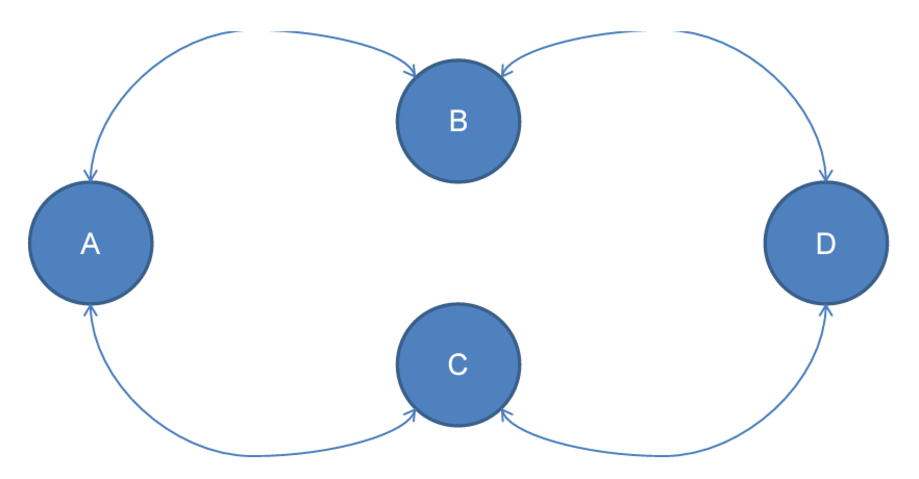
\includegraphics[width=0.5\textheight]{img/contact_example_topology.pdf}
    \caption{4つのノードからなるDTNの例}
    \label{fig:contact_example_topology}
    \begin{minipage}{\textwidth}
        \centering
        参考文献\cite{schedule_aware_bundle_routing}figure3-1より引用
    \end{minipage}
\end{figure}
\begin{figure}[tbh]
    \centering
    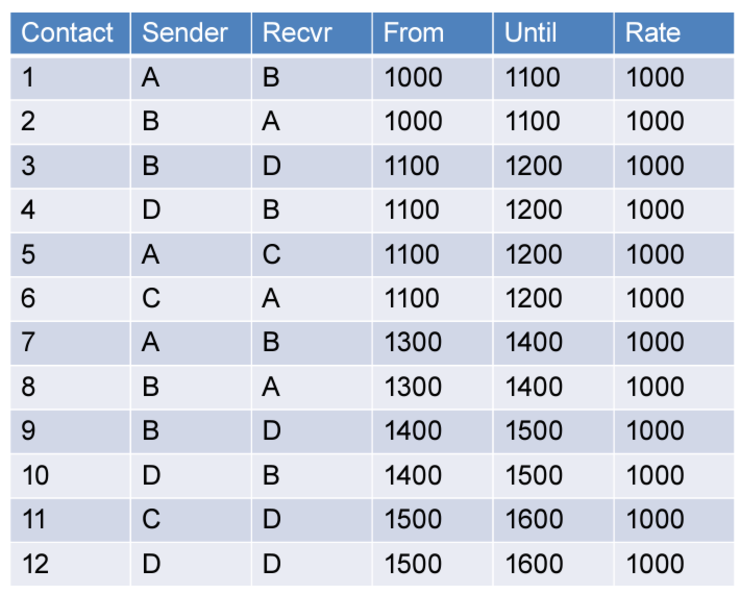
\includegraphics[width=0.5\textheight]{img/contact_example_contactplan.pdf}
    \caption{\ref{fig:contact_example_topology}におけるContact Planの例(Contactに関する表記)}
    \label{fig:contact_example_contactplan}
    \begin{minipage}{\textwidth}
        \raggedright
        参考文献\cite{schedule_aware_bundle_routing}figure3-2より引用。Senderは送信元のノードの識別子、Receiverは受信元のノードの識別子、FromはContactの開始時刻、Untilは終了時刻、Rateは転送速度を示す。
    \end{minipage}
\end{figure}
\begin{figure}[tbh]
    \centering
    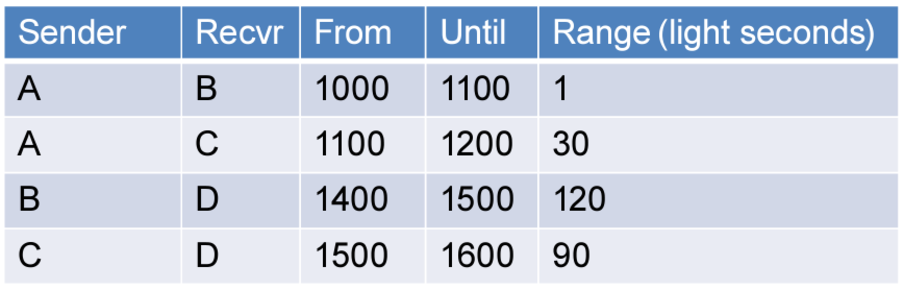
\includegraphics[width=0.5\textheight]{img/contact_example_contactrange.pdf}
    \caption{\ref{fig:contact_example_topology}におけるContact Planの例(Rangeに関する表記)}
    \label{fig:contact_example_contactrange}
    \begin{minipage}{\textwidth}
        \centering
        参考文献\cite{schedule_aware_bundle_routing}figure3-3より引用。
    \end{minipage}
\end{figure}
\begin{figure}[tbh]
    \centering
    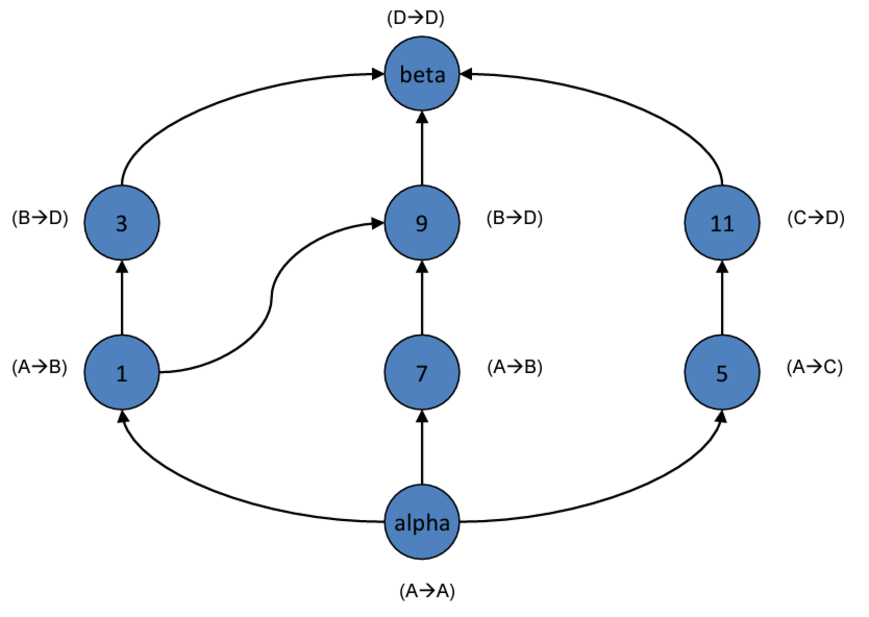
\includegraphics[width=0.5\textheight]{img/contact_example_contactgraph.pdf}
    \caption{\ref{fig:contact_example_topology}におけるContact Graphの例}
    \label{fig:contact_example_contactgraph}
    \begin{minipage}{\textwidth}
        \centering
        参考文献\cite{schedule_aware_bundle_routing}figure3-4より引用。
    \end{minipage}
\end{figure}